\part*{چند چارچوب و ابزار توسعه}
\chapter*{چند چارچوب و ابزار توسعه}
در فصل‌های قبلی تا قبل از این فصل تقریباً سندباکسی که برای استفاده مد نظر داشتیم، کامل شد، یعنی به راحتی می‌توانید در آن وردپرس، جوملا یا دروپال را که سامانه‌های مدیریت محتوا هستند را نصب کنید. با این وجود اگر در پیدا کردن فصل‌های قبلی دچار مشکل هستید، می‌توانید پیوند به آنان را در پایان این نوشته مشاهده کنید و از طریق آنان به فصل‌های قبلی رجوع کنید. در فصل قبل به بررسی نحوهٔ نصب برخی ماژول‌ها و ابزار مورد نیاز پرداختیم و در آخر نحوهٔ نصب و استفاده از یک گیت‌سرور ساده و آسان برای مدیریت پروژه‌ها را بررسی کردیم. در فصل پنجم، پیشخوان را از طریق گیت مدیریت کرده و توانستیم به موارد مختلفی چون تاریخچه و … در گیت دسترسی داشته باشیم.

در این فصل چند ابزار و چارچوب کاری برای کار با پی‌اچ‌پی «PHP»  را معرفی می‌کنیم و چند ابزار برای رفع ایراد و اشکال‌زدایی از کدهایتان را نیز بررسی خواهیم کرد. این فصل آخرین فصل از این مجموعهٔ آموزشی است و بعد از این فصل قرار است نسخهٔ پی‌اچ‌پی این مجموعه که با استفاده اززی‌لاتک ایجاد شده است را در اختیار شما دوستان قرار خواهیم داد. این فصل به صورت متن‌باز خواهد بود و زمان عرضهٔ آن در اسرع وقت خواهد بود. با این وجود برخی تغییرات نیز در نسخهٔ پی‌دی‌اف ممکن است به وجود آید که طبیعی است.
\part*{نحوهٔ نصب و اجرای برخی چارچوب‌های کاری برای زبان پی‌آچ‌پی}
\section{چارچوب کاری سیمفونی «Symfony»}
این چارچوب‌کاری محبوب یک چارچوب‌کاری متن‌باز است که برای نوشتن نرم‌افزارهای مبتنی بر وب در زبان پی‌اچ‌پی کاربرد دارد. اگر از زبان پی‌اچ‌پی استفاده می‌کنید، به یقین نام این چارچوب‌کاری را نیز شنیده‌اید. این چارچوب افزون بر ویژگی‌های متنوعی که برای توسعه یک نرم‌افزار یا یک درگاه اطلاع‌رسانی یا حتی یک پایگاه اینترنتی قوی دارد، از انعطاف‌پزیری بالایی نیز برخوردار است.

در این قسمت قصد داریم این چارچوب‌کاری و هم چارچوب‌کاری کیک‌-پی‌اچ‌پی ر نصب کنیم، برای نصب سیمفونی می‌توان از چندین روش استفاده کرد که یکی از  این روش‌ها،  در این نوشته بررسی می‌شود.

سیمفونی (به انگلیسی: 
\lr{Symfony}
) یک چارچوب نرم‌افزاری تحت وب متن‌باز است که برای ساخت وب‌گاه‌ها پویا به‌کار می‌رود. این چارچوب که با زبان پی‌اچ‌پی نوشته شده‌است، کار توسعهٔ نرم‌افزار را در سنجش با کد نویسی از آغاز شتاب می‌بخشد. این شتاب‌بخشی توسط کتابخانه‌های این چارچوب انجام می‌شود که بسیاری از آنها کارهای رایج را بسادگی انجام می‌دهند. این چارچوب بر اساس مدل معماری مدل-نما-کنترل‌گر (به انگلیسی: 
\lr{MVC}
) کار می کند.این چارچوب پیاده سازی های شما را بر اساس بسته های (به انگلیسی: 
\lr{bundle}
) ایجاد کرده پیش خواهد برد و شما نیز می تواند از هزاران بسته نوشته شده متن باز دیگران در پروژه خود استفاده کنید. 
\begin{flushleft}
    (ویکی‌پدیا، دانشنامه آزاد)
\end{flushleft}

برای نصب این چارچوب‌کاری ما از ابزار «composer» استفاده می‌کنیم، اگر این ابزار در توزیع شما نصب نیست به قسمت پنجم این مجموعهٔ آموزشی مراجعه کرده و آن را نصب کنید. برای نصب آن از طریق «composer» دستورات زیر را در خط فرمان اوبونتو سرور، اجرا کنید.
\newline

\begin{latin}  
    \lstinputlisting[numbers=right,language=SH, framexleftmargin=5mm, frame=shadowbox,rulesepcolor=\color{Black}]{Code/framework.sh}
\end{latin}

سپس هر آنچه را که از شما پرسیده می‌شود را مطابق موردی که در زیر آمده است، پر کنید. در این تنظیمات می‌توانید از پایگاه داده‌ای جدا همنام با سیمفونی استفاده کنید که پیشنهاد ما نیز همین است، با این حال می‌توانید از کاربر و پایگاه‌دادهٔ سندباکس که در قسمت‌های قبلی ساخته‌ایم استفاده کنید.
\newline

\begin{latin}  
    \lstinputlisting[numbers=right,language=SH, framexleftmargin=5mm, frame=shadowbox,rulesepcolor=\color{Black}]{Code/framework.txt}
\end{latin}

سپس باید پروندهٔ 
\path{«ap_dev.php»} 
را از داخل پوشهٔ سیمفونی گشوده و مقادیر زیر را جایگزین آن نمایید. در این پرونده تغییراتی را اعمال کرده‌ایم، که فقط زمانی که از 
\path{«sandbox.dev»}
 به عنوان آدرس برای ورود به صفحهٔ مدیریت و توسعه سیمفونی شدیم، محیط چارچوب‌کاری سیمفونی اجرا شود. برای همین دیگر شروط که ممکن است نرم‌افزار را دچار مشکل کند را حذف کرده‌ایم.

برای ایجاد تغییرات در آن، ابتدا باید نرم‌افزار اتم «Atom» یا هر ویرایشگر یا محیط توسعه‌ای را که دوست دارید را اجرا کنید  و پوشهٔ «symfony» که در پوشهٔ  سندباکس «Sandbox»  قرار دارد را در آن نرم‌افزار بگشایید. به عنوان مثال در تصویر \ref{ATOM-FRAMEWORK} ویرایشگر اتم «Atom» را مشاهده می‌کنید. 

\begin{latin}  
    \lstinputlisting[numbers=right,language=PHP, framexleftmargin=5mm, frame=shadowbox,rulesepcolor=\color{Blue}]{Code/symfony-conf.php}
\end{latin}
\begin{figure}
    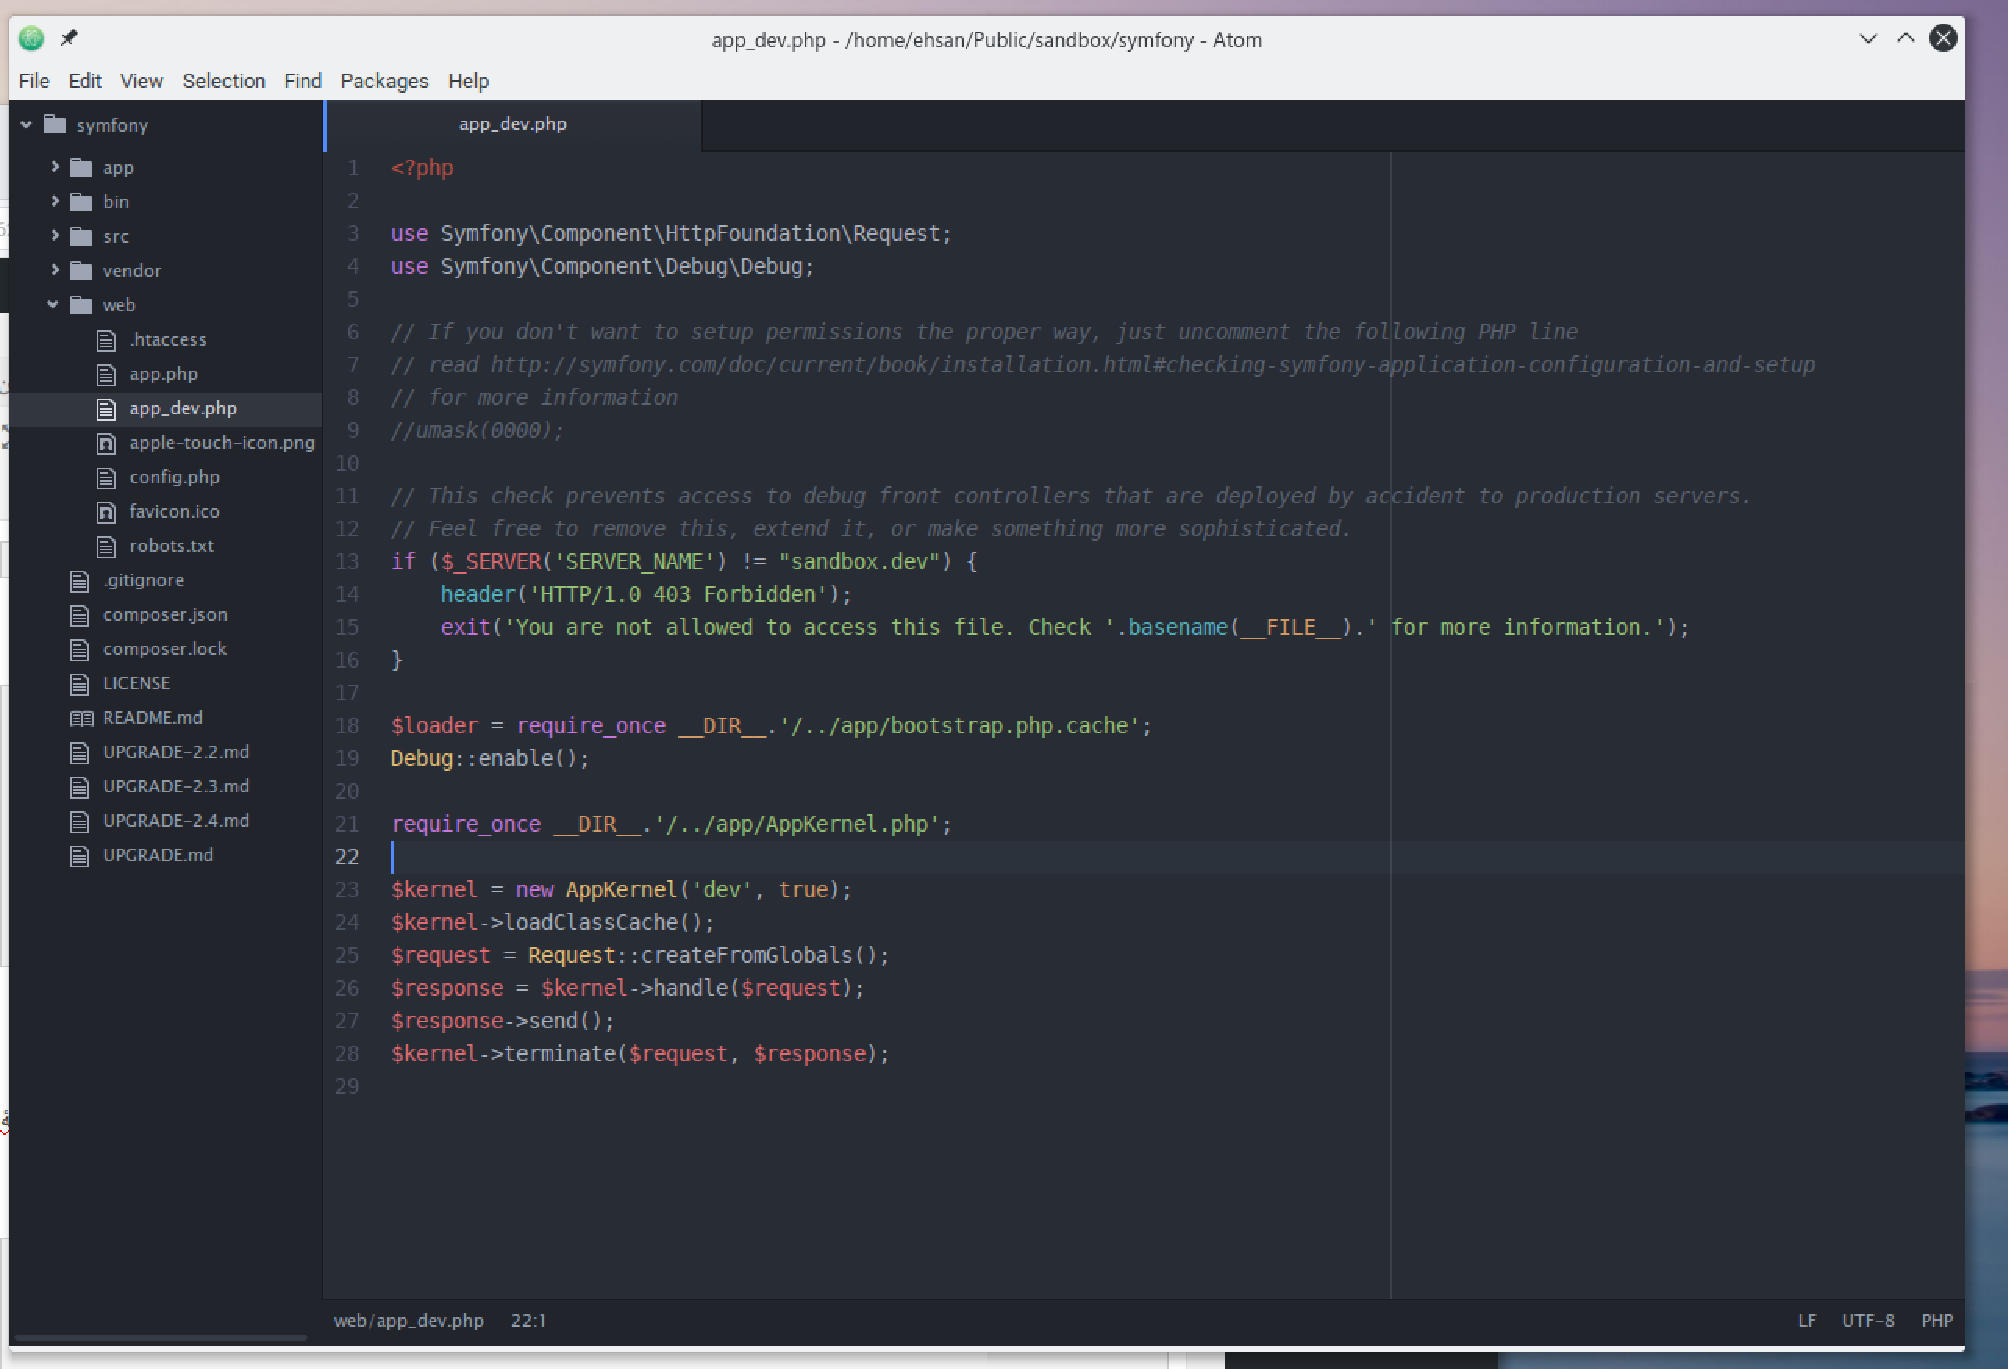
\includegraphics[width=.9\textwidth ,height=.65\textwidth]{Pic/FRAME-WORK-ATOM}
    \caption{ ویرایش تنظیمات سیمفونی 
        \lr{Symfony's Config file | }   
    }
    \label{ATOM-FRAMEWORK}
\end{figure}

بعد از این تغییرات اگر به آدرس زیر مراجعه کنید با صفحه‌ای مشابه با تصویر مواجه شده و بعد از آن به راحتی خواهید توانست از این چارچوب‌کاری برای توسعه نرم‌افزارهای پی‌اچ‌پی و یا پایگاه‌های اینترنتی خود استفاده کنید. کاربرد این چارچوب‌کاری بسیار گسترده است، اگر از مطلبی برای آموزش و یادگیری این چارچوب‌‌کاری بهره می‌گیرید، نیاز به محیطی برای نوشتن کد و یادگیری دارید.   بنابراین با استفاده از این سندباکس می‌توانید این چارچوب را نیز فرا بگیرید.
\newline
\begin{latin}  
    \lstinputlisting[numbers=right,language=SH, framexleftmargin=5mm, frame=shadowbox,rulesepcolor=\color{Black}]{Code/symfony-url.txt}
\end{latin}

\begin{figure}
    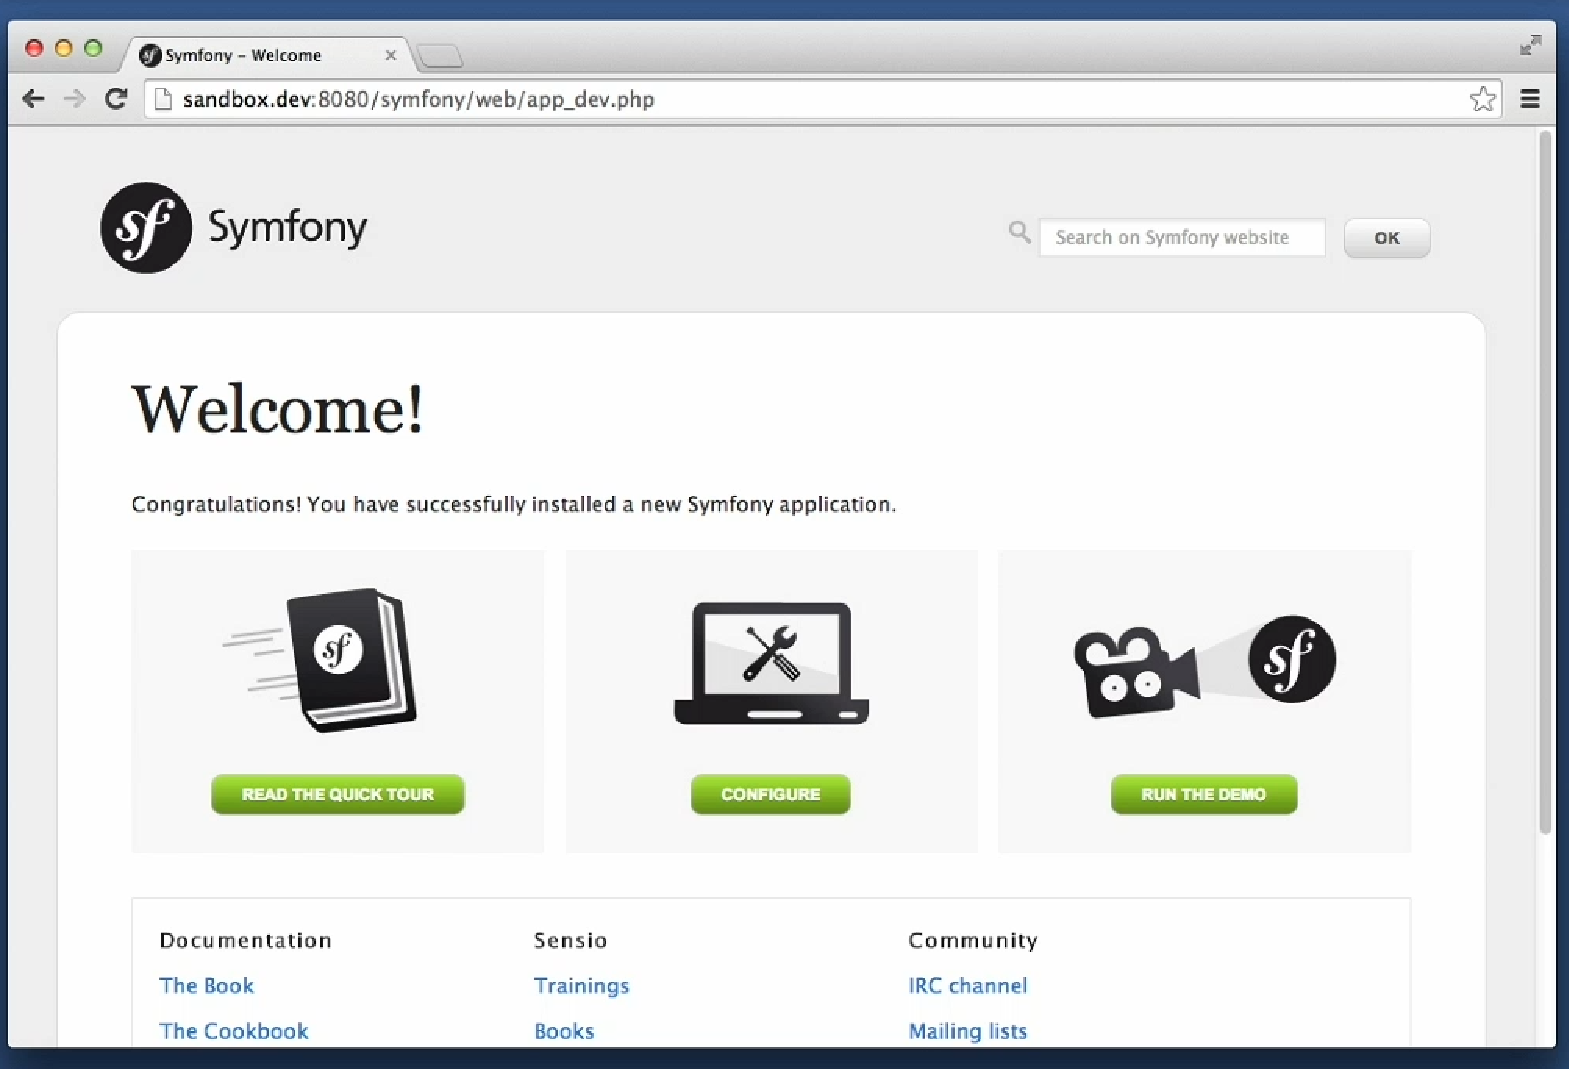
\includegraphics[width=.9\textwidth ,height=.65\textwidth]{Pic/SYMFONY-PAGE}
    \caption{ نمایی از چارچوب کاری  سیمفونی 
        \lr{Symfony | }   
    }
    \label{SYMFONY-FRAMEWORK}
\end{figure}

\section{چارچوب‌کاری کیک پی‌اچ‌پی CackePHP}

این چارچوب کاری نیز یک چارچوب کاری متن‌باز و آزاد است، این چارچوب‌کاری نیز محبوب بوده و توسط کاربران و توسعه‌دهندگان مختلف پی‌اچ‌پی استفاده می‌شود.  در این قمست به نحوهٔ نصب و اجرای این چارچوب‌کاری در سندباکس خواهیم پرداخت،  مسائلی مانند تنظیم پایگاه داده یا پرونده‌هایی که برای تنظیم این چارچوب‌کاری باید تغییر یابند را از این قسمت با هم بررسی می‌کنیم.

کیک‌پی‌اچ‌پی (به انگلیسی: 
\lr{CakePHP}
) یک چارچوب نرم‌افزاری تحت وب آزاد برای تولید برنامه‌های وب است که به زبان پی‌اچ‌پی نوشته شده‌است. این چارچوب از معماری مدل-نما-کنترل‌گر پیروی می‌کند و شی گرا است که تحت اجازه‌نامهٔ ام‌آی‌تی منتشر می‌شود. 

\begin{flushleft}
    (ویکی‌پدیا، دانشنامه آزاد)
\end{flushleft}

برای نصب آن، ابتدا باید به شاخه‌ای که برای نگهداری پرونده‌ها و پوشه‌هایمان به نام Sandbox ایجاد کرده بودیم و در ویرچوال‌باکس به اشتراک گذاشتیم، شویم و در داخل آن پوشه،  دستورات مناسب برای نصب این چارچوب‌کاری را در خط فرمان وارد کنیم.

\begin{latin}  
    \lstinputlisting[numbers=right,language=SH, framexleftmargin=5mm, frame=shadowbox,rulesepcolor=\color{Black}]{Code/cakephp.sh}
\end{latin}

حالا و بعد از ورود به شاخهٔ بالا، با استفاده از مدیر نصب ماژول و اجراء جدید خط فرمانی «Composer»  می‌توانیم پروندهٔ مورد نیاز برای نصب این چارچوب کاری را بارگیری کنیم، برای بارگیری پروندهٔ آرشیو این چارچوب‌کاری دستور زیر را در خط فرمان وارد کنید. در هنگامی که از شما سوالی پرسیده شد حرف وای را به صورت بزرگ «Y» را نوشته و کلید اینتر روی صفحه کلید را فشار دهید.
\begin{latin}  
    \lstinputlisting[numbers=right,language=SH, framexleftmargin=5mm, frame=shadowbox,rulesepcolor=\color{Black}]{Code/cakephp2.sh}
\end{latin}
بعد از اینکه همه چیز به خوبی نصب شد، تقریباً تمامی مراحل نصب کیک‌پی‌اچ‌پی به پایان رسیده است به جز این مورد که در کیک‌پی‌اچ‌پی «CakePHP» تنظیمات پایگاه داده انجام نشده است، وارد نرم‌افزار مدیریت MySQL مانند PHPMyAdmin شده و یک حساب کاربری به همراه یک پایگاه داده مشابه با نام آن ایجاد کنید تا برای استفاده در کیک‌پی‌اچ‌پی از آن استفاده کنیم. بعد از اینکه ابزار مورد اشاره نصب شد،ب بیایید تا ابزار دیباگ-کیت «DebugKIT» را هم که ابزاری برای مدیریت خطا و ایراد و اشکال‌زدایی است را نیز نصب کنیم. برای نصب کیک-پی‌اچ‌پی از طریق «Composer» دستورات زیر را در خط فرمان وارد کنید.
\begin{latin}  
    \lstinputlisting[numbers=right,language=SH, framexleftmargin=5mm, frame=shadowbox,rulesepcolor=\color{Black}]{Code/cakephp3.sh}
\end{latin}

این ابزار نیز توسط همان تیمی که کیک‌پی‌اچ‌پی را توسعه می‌دهند نوشته شده است و برای رفع ایراد و … در هنگام نوشتن کدهای پی‌اچ‌پی گزینهٔ مناسبی است و با کیک‌پی‌اچ‌پی «CakePHP»  هماهنگی خوبی دارد. این کار باید در داخل خود پوشهٔ کیک‌-پی‌اچ‌پی انجام شود. برای تنظیم کردن این چارچوب‌کاری همانند چارچوب کاری سیمفونی، پوشهٔ  «cakephp»  را در دخل محیط توسعه یا ویرایشگر متنی مانند اتم «Atom» گشوده و تغییرات را در آن اعمال می‌کنیم.  (همانند تصویر \ref{CAKEPHP-ATOM-FRAMEWORK})
\begin{figure}
    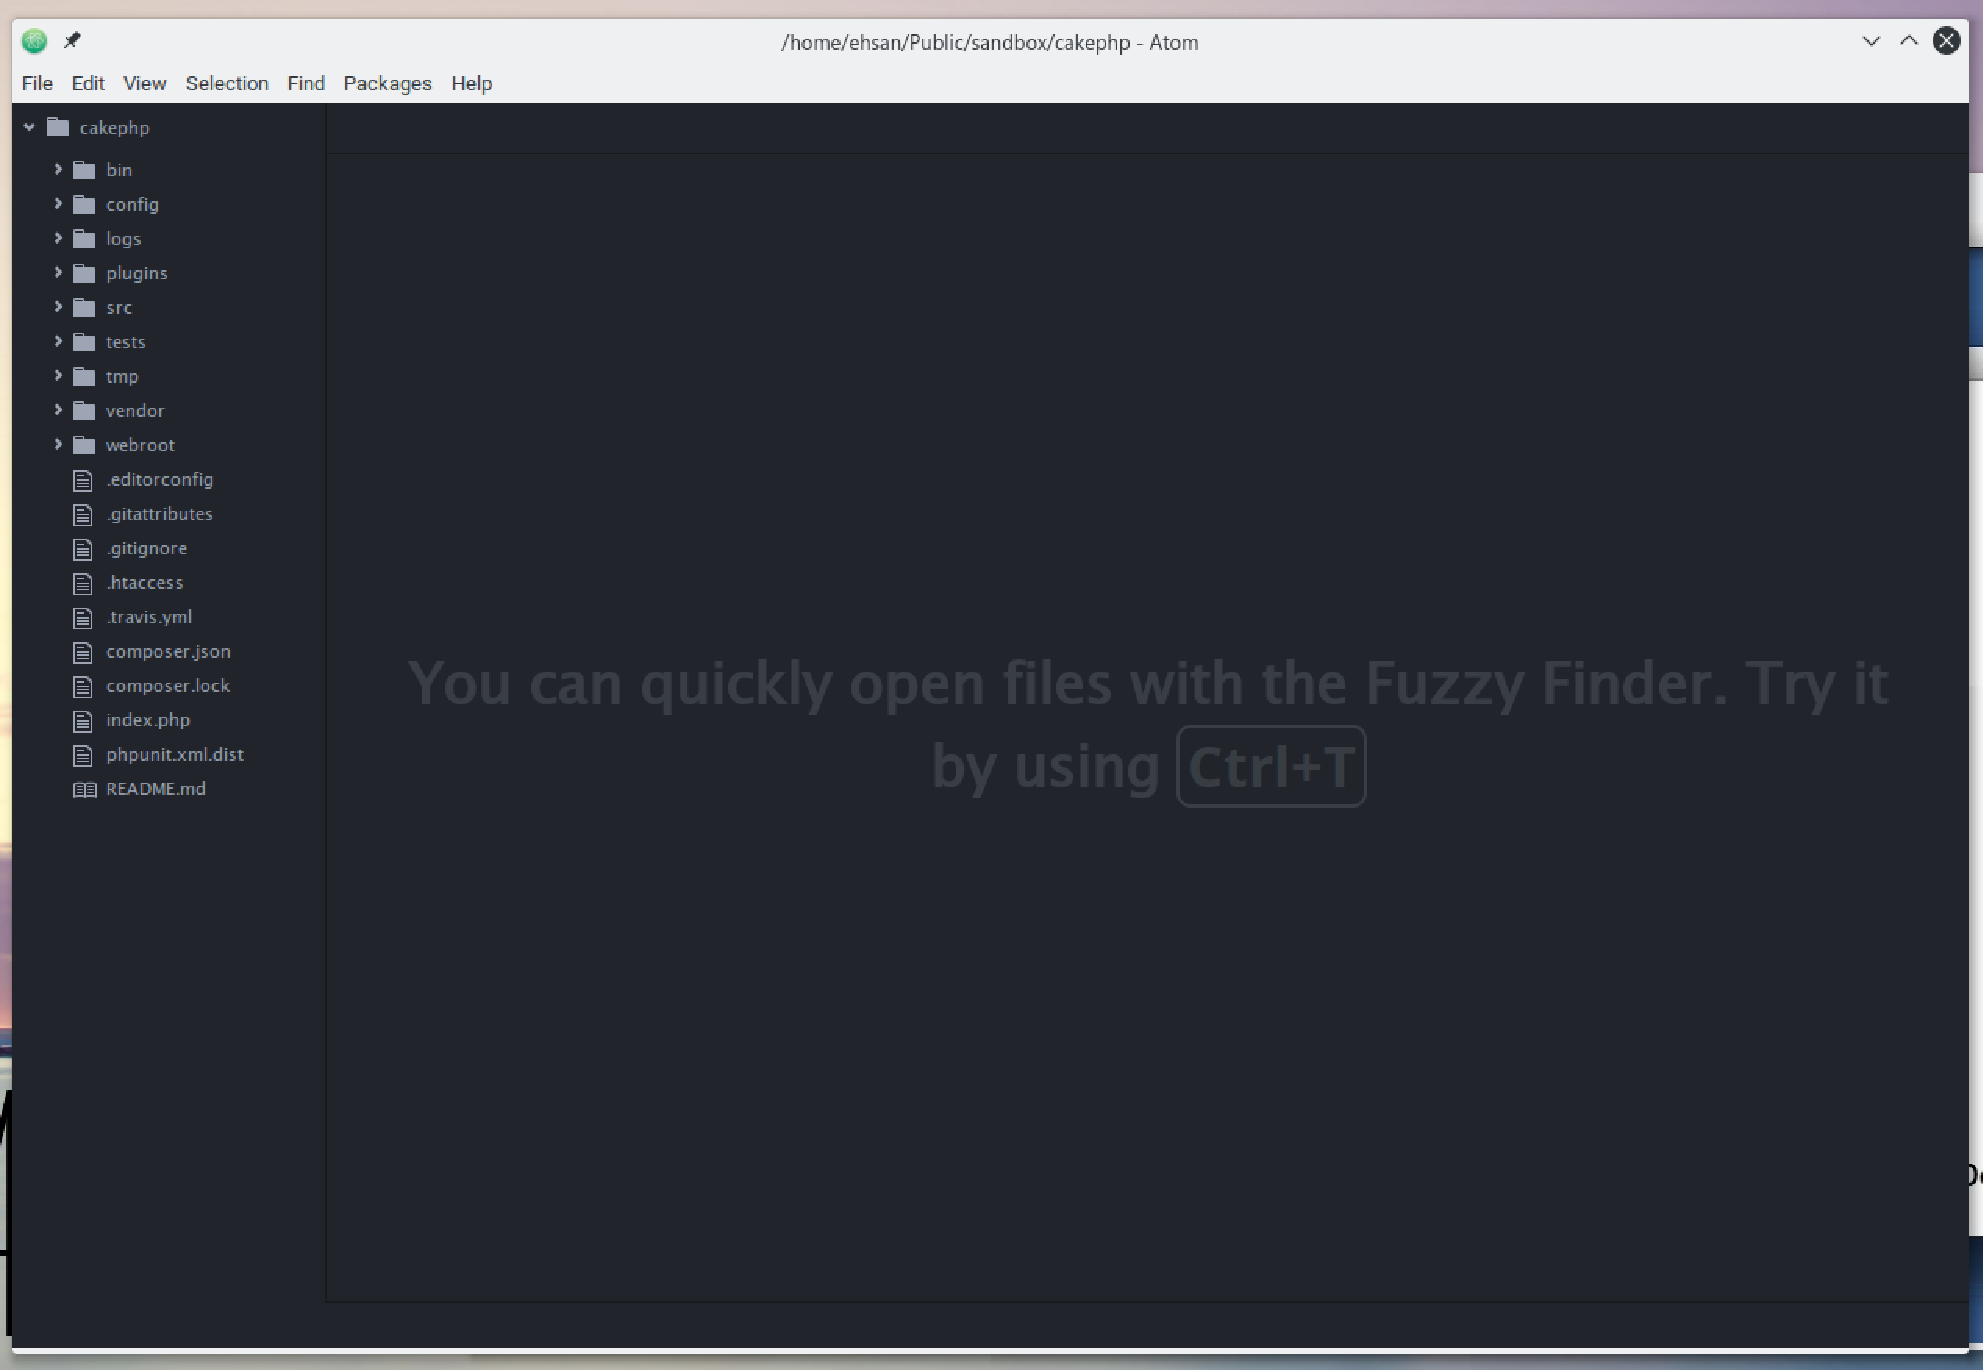
\includegraphics[width=.9\textwidth ,height=.65\textwidth]{Pic/CAKEPHP-ATOM}
    \caption{ ویرایش تنظیمات چارچوب کاری
        \lr{CakePHP | }   
    }
    \label{CAKEPHP-ATOM-FRAMEWORK}
\end{figure}

از طریق قسمتی که برای مشاهدهٔ پوشه‌ها و پرونده‌ها در کیک‌پی‌اچ‌پی قرار دارد به راحتی می‌توانید پوشه‌ها و پرونده‌های نصب شده را مشاهده کنید. به پوشهٔ «cakephp» در پوشهٔ اشتراکی سندباکس خود رفته و در پوشهٔ داخل آن با نام «Config» پروندهٔ «app.php» را بگشایید. به خطوطی که در آن مقادیری به شکل نامعلوم و گنگ نوشته شده رفته و مقادیری که برای امنیت به صورت تصادفی نوشته شده است را به مورد دیگری تغییر دهید تا در حالت پیش‌فرض نباشند. (مانند تصویر \ref{CAKEPHP-ATOM-FRAMEWORK2})

\begin{figure}
    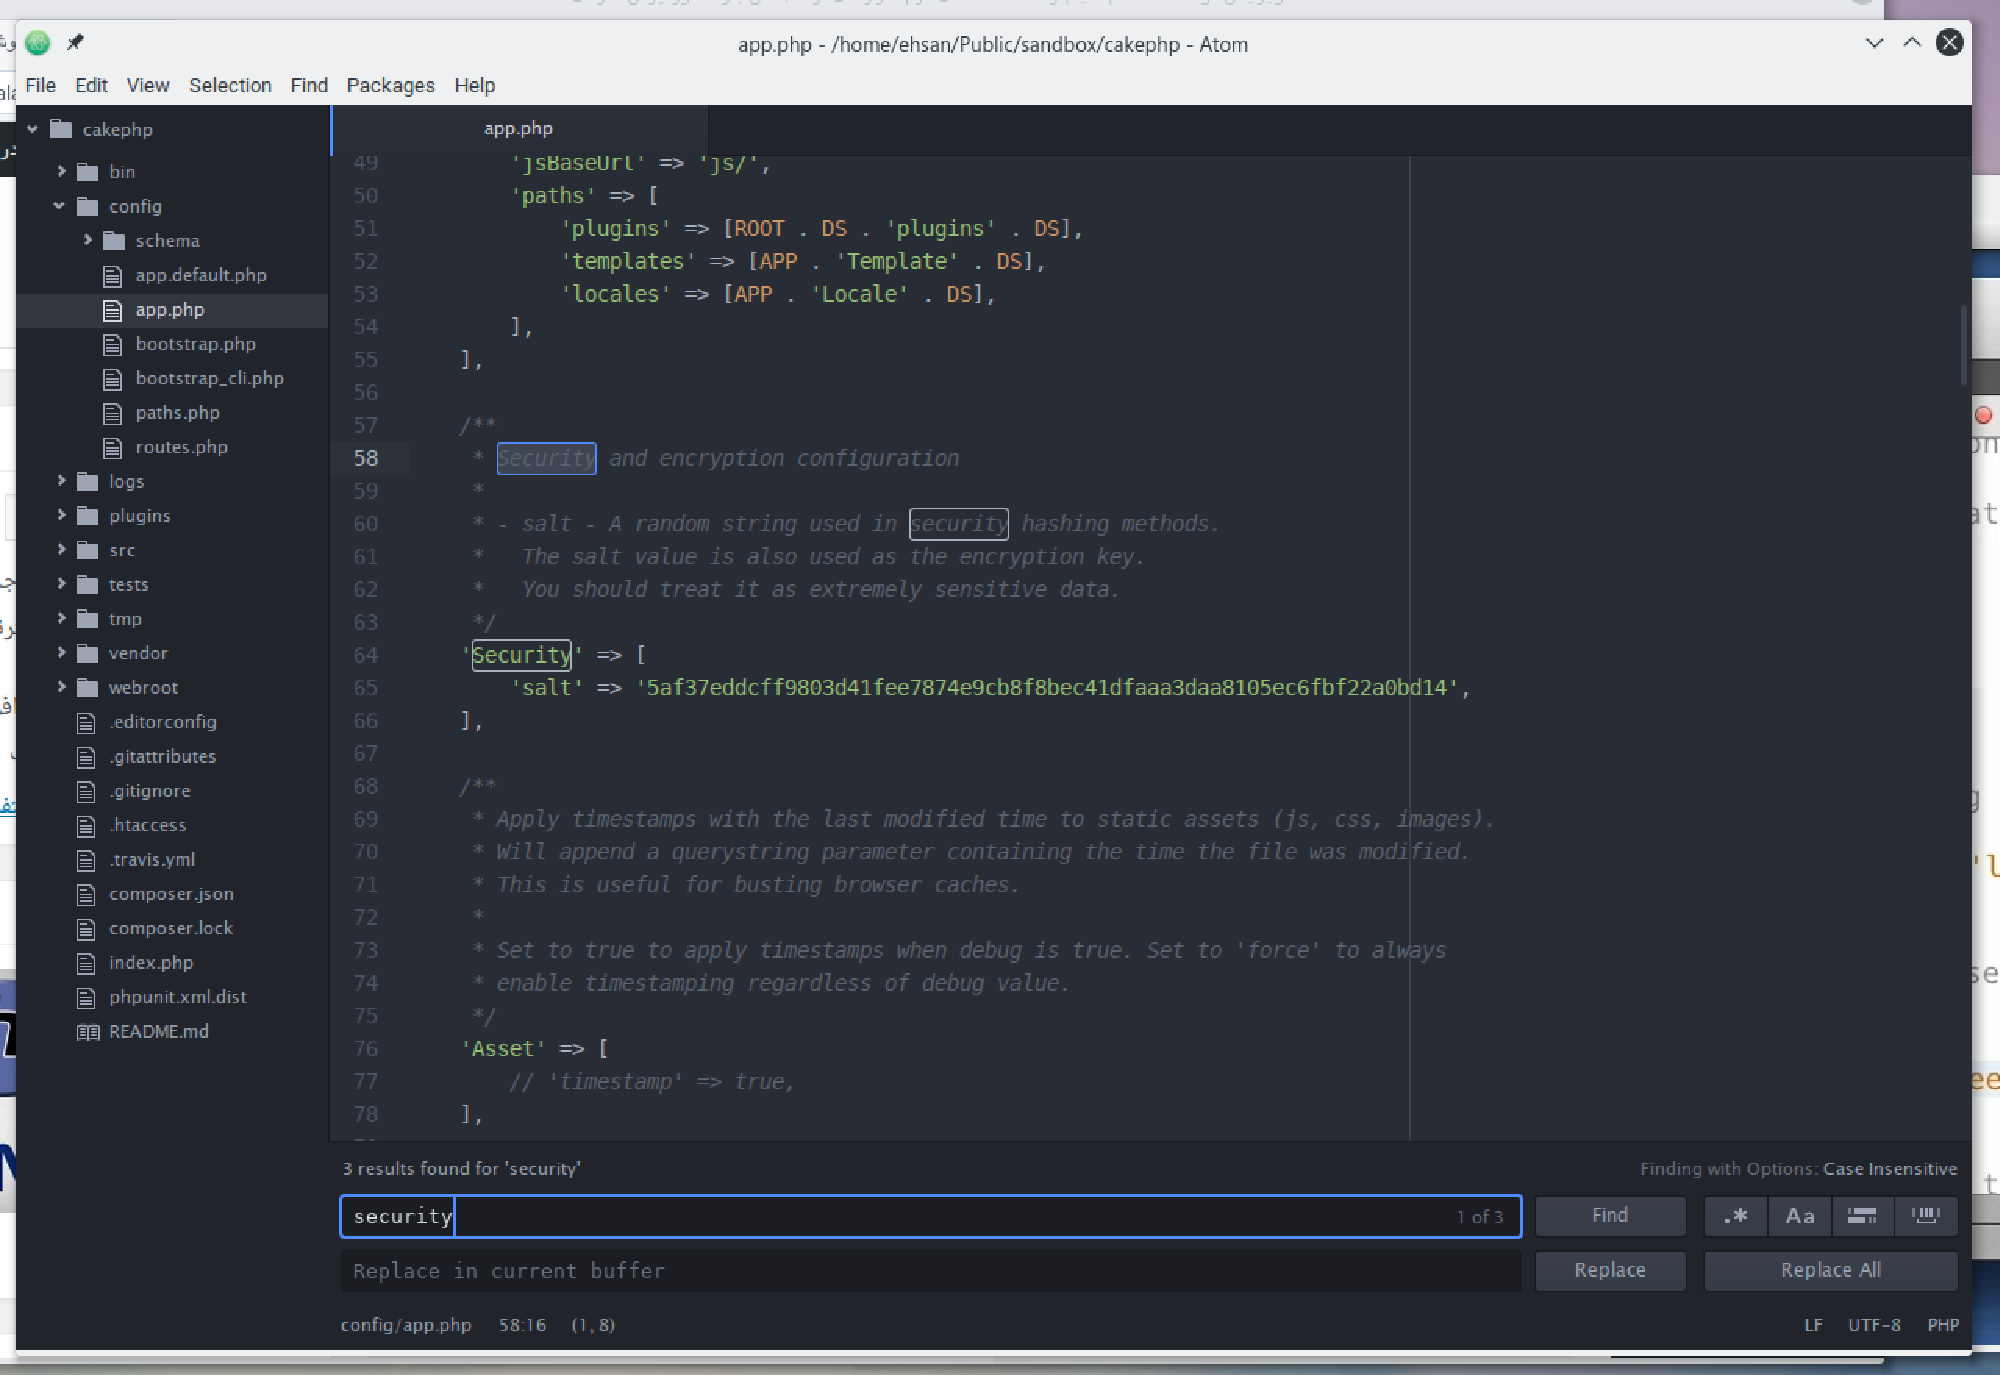
\includegraphics[width=.9\textwidth ,height=.65\textwidth]{Pic/CAKEPHP-ATOM2}
    \caption{ ویرایش اعداد تصادفی در تنظیمات چارچوب کاری
        \lr{CakePHP | }   
    }
    \label{CAKEPHP-ATOM-FRAMEWORK2}
\end{figure}

حال برای تنظیم پایگاه داده به خط 218 در همان فایل رفته و مقادیری که برای اتصال به پایگاه داده لازم است را تصحیح کنید. در آن ما نام کاربری مورد نظر خود را در مای‌اس‌کیوال به همراه گذرواژه بنویسید.
\begin{latin}  
    \lstinputlisting[numbers=right,language=PHP, framexleftmargin=5mm, frame=shadowbox,rulesepcolor=\color{Blue}]{Code/cakephp4.php}
\end{latin}
بعد از این، خطوط 249 به بعد را نیز به همان ترتیب بالا تغییر دهید.  حال برای فعال کردن دیباگ-کیت خط زیر را نیز به این پرونده اضافه کنید.

\begin{latin}  
    \lstinputlisting[numbers=right,language=PHP, framexleftmargin=5mm, frame=shadowbox,rulesepcolor=\color{Blue}]{Code/cakephp5.php}
\end{latin}
حال اگر وارد آدرس زیر شوید، کیک-پی‌اچ‌پی «CakePHP» به خوبی اجرا شده و خطایی در آن مشاهده نخواهید کرد. حال یا استفاده از این چارچوب‌کاری می‌توانید نرم‌افزارهای و صفحات مورد نظر خود را طراحی و توسعه دهید.
\begin{figure}
    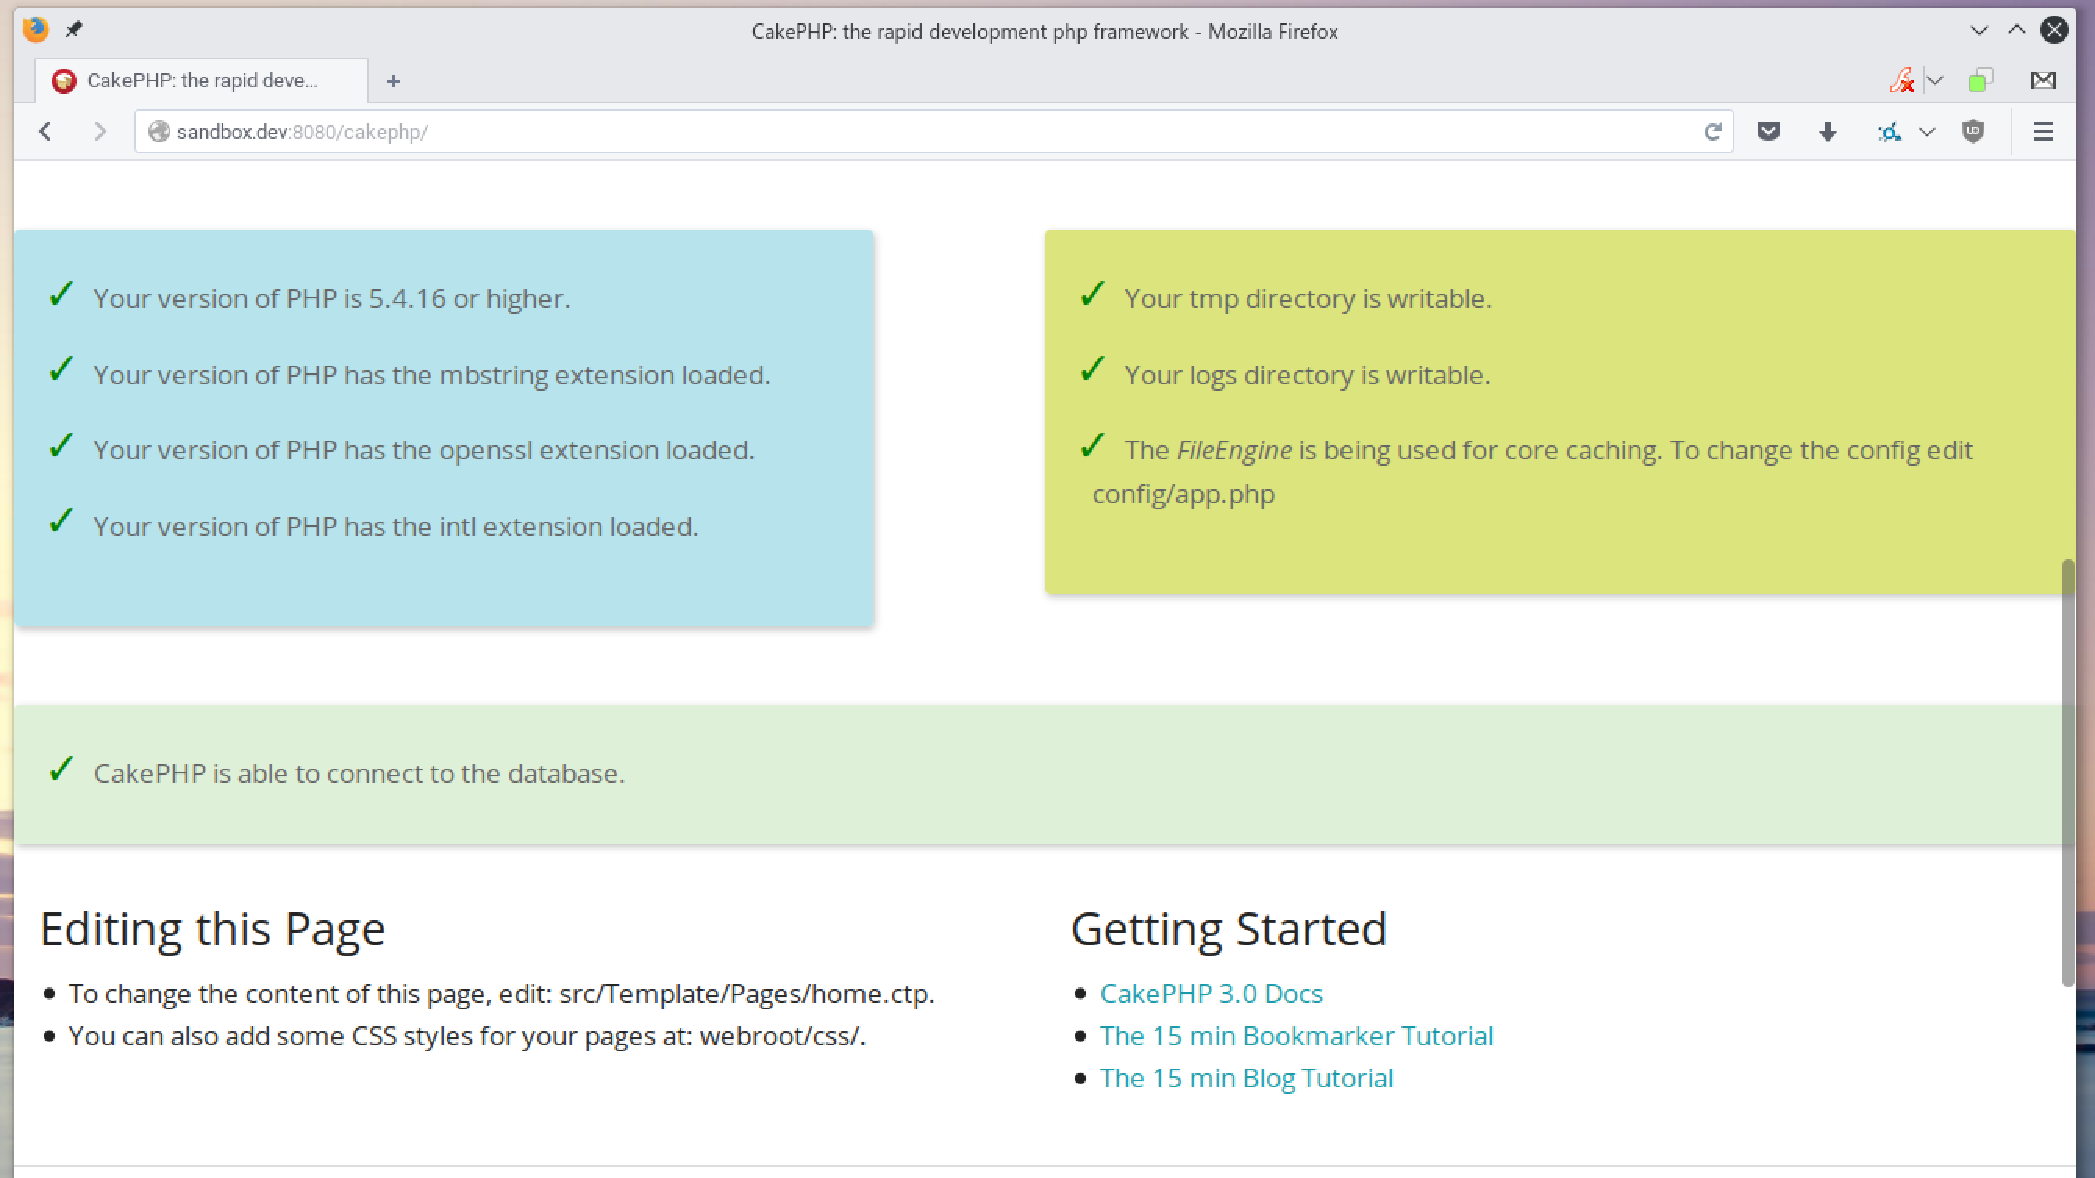
\includegraphics[width=.9\textwidth ,height=.55\textwidth]{Pic/CAKEPHP}
    \caption{ نمایی از چارچوب چارچوب کاری
        \lr{CakePHP }
        که به خوبی تنظیم شده است.   
    }
    \label{CAKEPHP-FRAMEWORK-PAGE}
\end{figure}